\chapter{User Management and Authentication}

\section{Introduction}

This chapter presents the implementation of user management and authentication functionalities, which constitute the foundation of the platform. These components ensure secure access control, enforce enterprise-level restrictions, and enable structured interactions between users and the system.

The implementation corresponds to \textbf{Sprint 1} within the Agile development process. This sprint focuses on establishing a reliable authentication mechanism based on enterprise credentials, managing user profiles, and providing administrative control features. All functionalities were developed incrementally and validated at the end of the sprint to ensure correctness and system stability.

\section{Sprint 1: User Management and Authentication}

\subsection{Sprint Goal}

The objective of this sprint is to implement a secure and controlled access mechanism based on enterprise authentication while providing essential user management functionalities. This includes profile handling, role-based access control, and administrative supervision capabilities.

This sprint is critical as it establishes the security backbone of the system and ensures that only authorized users can access platform functionalities.

\subsection{Product Backlog}

\begin{table}[H]
\centering
\begin{tabular}{|l|l|l|l|}
\hline
\textbf{ID} & \textbf{User Story} & \textbf{Actor} & \textbf{Priority} \\
\hline
US1 & Authenticate using Office 365 account & Collaborator & High \\
US2 & Restrict access to @gexpertise.fr domain & System & High \\
US3 & View personal profile & Collaborator & Medium \\
US4 & Update profile information & Collaborator & Medium \\
US5 & Monitor user activity & Admin & High \\
US6 & Freeze or restrict user account & Admin & High \\
\hline
\end{tabular}
\caption{Sprint 1 Product Backlog}
\end{table}

The prioritization reflects the critical importance of security and access control. Authentication and domain restriction are classified as high priority as they prevent unauthorized access. Administrative functionalities are also prioritized to ensure system integrity and control, while profile-related features are considered secondary but necessary for user interaction.

\subsection{Use Case Diagram}

\begin{figure}[H]
    \centering
    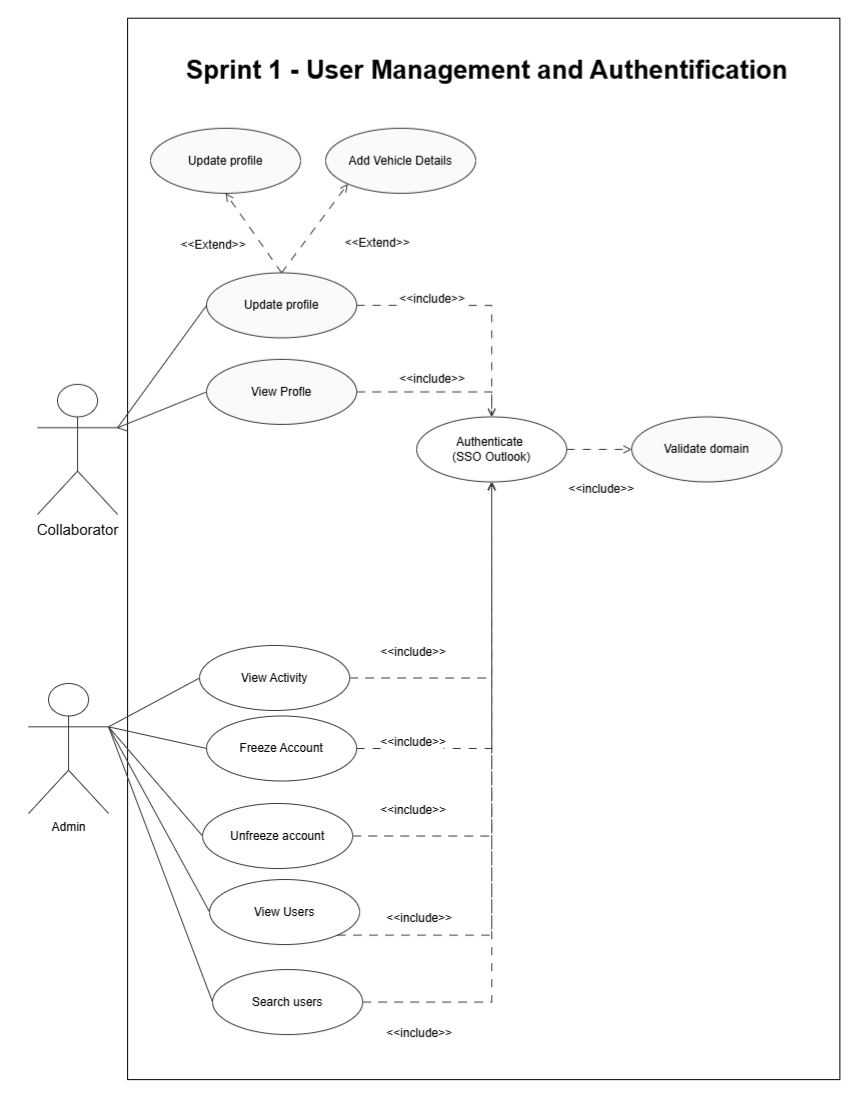
\includegraphics[width=0.4\textwidth]{images/diagrams/use_case_sprint2.png}
    \caption{Use Case Diagram - User Management}
\end{figure}

The use case diagram illustrates the interactions between system actors and the platform functionalities. Two primary actors are identified: the \textbf{Collaborator}, representing the standard user, and the \textbf{Administrator}, responsible for system supervision.

Authentication is a prerequisite for most operations, ensuring that access is restricted to authorized users. Profile-related actions such as viewing and updating information are independent functionalities, reflecting user autonomy. Administrative actions, including monitoring activity and managing user accounts, highlight the role of the administrator in maintaining system integrity.

\subsection{Sequence Diagram}

\begin{figure}[H]
    \centering
    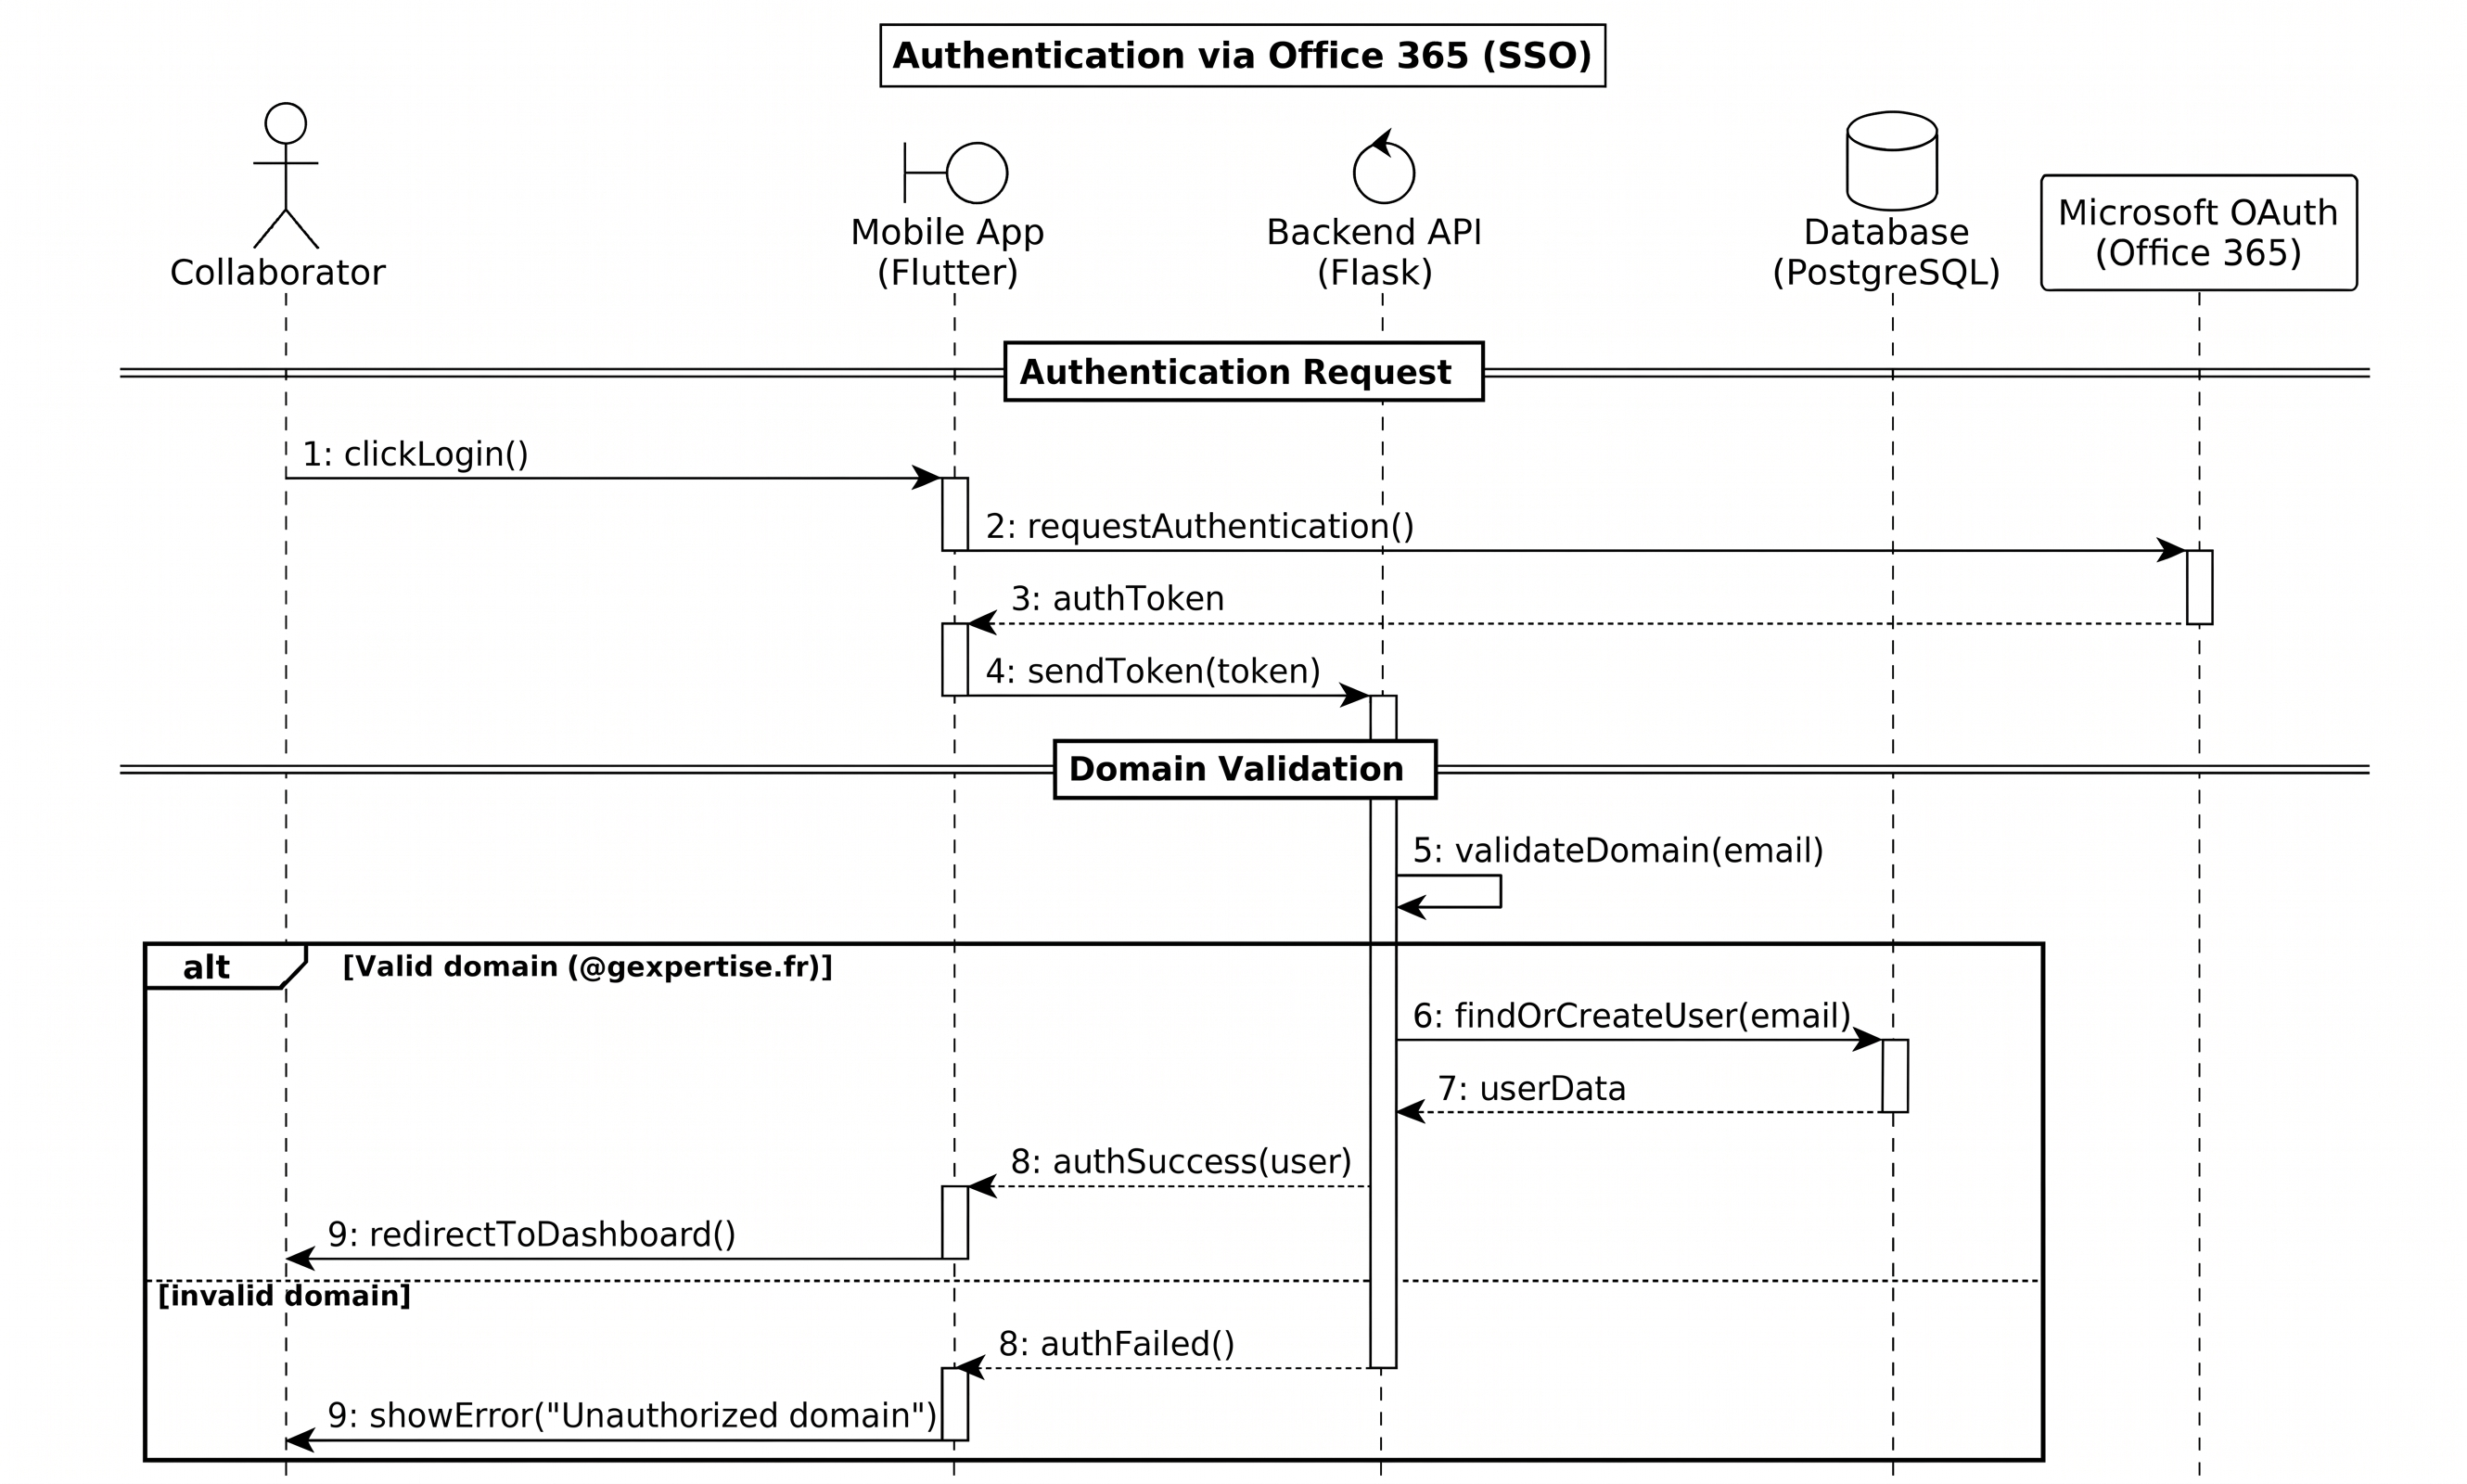
\includegraphics[width=0.7\textwidth]{images/diagrams/sequence_auth.png}
    \caption{Authentication Sequence Diagram}
\end{figure}

The sequence diagram describes the dynamic interaction between system components during the authentication process. It highlights the integration of external identity providers with internal system validation.

The authentication workflow follows these steps:

\begin{enumerate}
    \item The user initiates the authentication process from the mobile application.
    \item The application redirects the request to the Microsoft Office 365 authentication provider.
    \item Upon successful authentication, an access token is returned to the client.
    \item The token is transmitted to the backend server for validation.
    \item The backend verifies the authenticity of the token and enforces domain-based access control.
    \item If the email domain is valid, the system retrieves or creates the user record in the database.
    \item A secure session is established, and the user is granted access to the platform.
\end{enumerate}

This design ensures a clear separation between authentication and application logic. By delegating identity verification to a trusted external provider and enforcing domain validation internally, the system guarantees both security and organizational control.

\subsection{Class Diagram}

\begin{figure}[H]
    \centering
    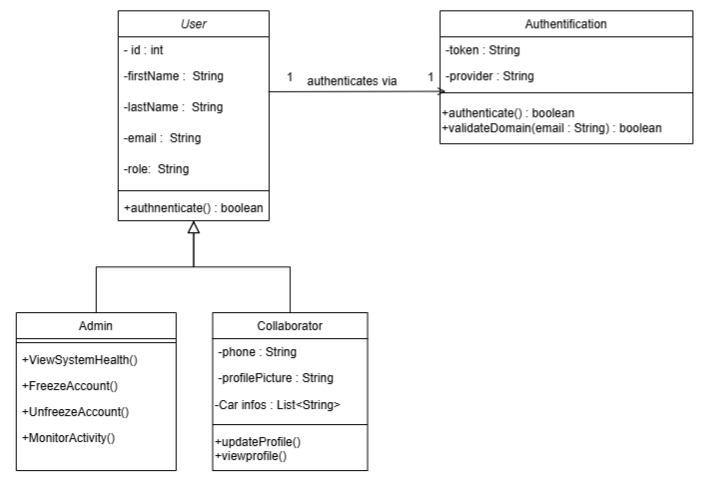
\includegraphics[width=0.6\textwidth]{images/diagrams/class_user.png}
    \caption{Class Diagram - User Domain}
\end{figure}

The class diagram represents the structural organization of user-related entities within the system.

The \textbf{User} class serves as the central entity and is specialized into two roles: \textbf{Collaborator} and \textbf{Administrator}. This inheritance structure reflects role-based access control, where each type of user has specific responsibilities and permissions.

The \textbf{Authentication} component is modeled as a separate entity to encapsulate authentication logic, including token management and domain validation. This separation improves modularity and allows authentication mechanisms to evolve independently from user management.

The administrator maintains control over user accounts, including monitoring activity and enforcing restrictions. This relationship ensures that the system remains secure and compliant with enterprise requirements.

\section{Authentication Mechanism}

Authentication is implemented using \textbf{Single Sign-On (SSO)} through Microsoft Office 365. This approach eliminates the need for manual registration and leverages an existing enterprise identity infrastructure.

Access is strictly restricted to users possessing a valid professional email address within the \textbf{@gexpertise.fr} domain. This constraint ensures that only authorized employees can access the platform, reinforcing organizational boundaries.

From an architectural perspective, authentication is divided into two phases:

\begin{itemize}
    \item \textbf{External Authentication:} Handled by Microsoft Office 365, responsible for verifying user identity.
    \item \textbf{Internal Validation:} Performed by the backend, responsible for enforcing domain restrictions and managing user records.
\end{itemize}

This dual-layer approach enhances security by combining trusted external identity management with application-level access control.

\begin{figure}[H]
    \centering
    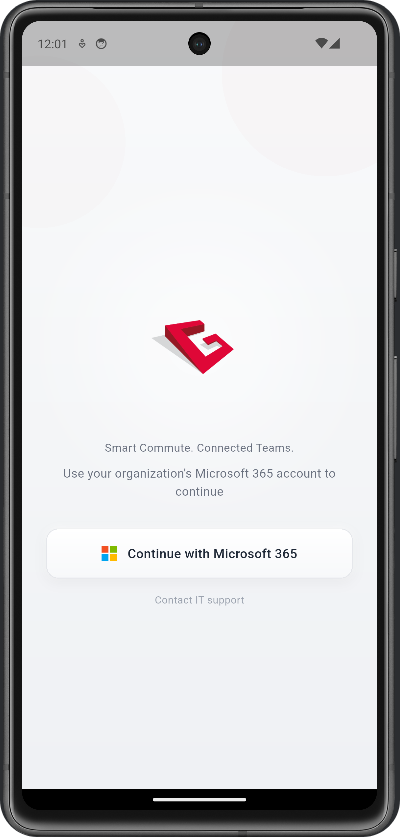
\includegraphics[width=0.3\textwidth]{images/ui/login_screen.png}
    \caption{Login Interface using Office 365}
\end{figure}

The user interface reflects this design by providing a single entry point through the Office 365 authentication system, ensuring a seamless and secure login experience.

\subsection{Enterprise Access Control Model}

The access control model implemented in this system is specifically designed for enterprise environments where user membership is strictly bounded by organizational affiliation. Unlike public platforms that accept arbitrary registrations, the proposed system enforces a closed population model in which access is contingent upon possession of a valid corporate identity.

This design choice carries three fundamental implications. First, the user base is inherently restricted to employees of the host organization, eliminating the need for external trust mechanisms such as ratings or third-party verification. Second, registration is not an open user action but a controlled system-side process triggered by successful enterprise authentication. The system either retrieves an existing record or creates a new one upon first login, ensuring that no user can exist in the database without prior organizational validation. Third, the platform operates under a role-based access control scheme where users are classified as either standard collaborators or administrators, with administrative privileges granting supervisory authority over accounts, activity monitoring, and system-wide policy enforcement.

This enterprise-oriented access model ensures system integrity by maintaining a controlled and verifiable user population. It reinforces administrative authority, simplifies security governance, and aligns the platform with the operational boundaries of the organization it serves.

\section{Profile Management}

Authenticated users can access and manage their personal profiles, which serve as the basis for personalization and interaction within the platform.

Users are able to:

\begin{itemize}
    \item View personal and professional information
    \item Update profile data such as contact details and vehicle information
\end{itemize}

All modifications are validated at the backend level before being persisted in the database. This validation process ensures data integrity, prevents inconsistencies, and maintains the reliability of user information.

\begin{figure}[H]
    \centering
    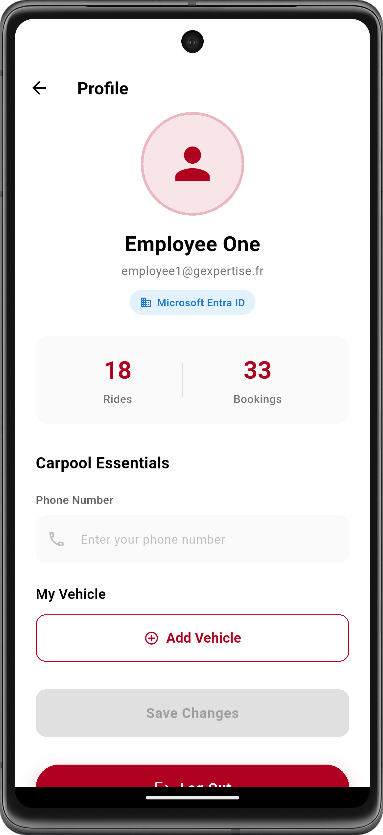
\includegraphics[width=0.3\textwidth]{images/ui/profile_screen.png}
    \caption{User Profile Interface}
\end{figure}

\section{Administrative Features}

Administrators play a fundamental role in maintaining system stability and enforcing platform policies. Their responsibilities extend beyond simple user interaction to include supervision and control mechanisms.

The platform provides the following administrative capabilities:

\begin{itemize}
    \item Monitoring user activity and system usage
    \item Detecting abnormal or suspicious behavior
    \item Freezing or restricting user accounts when necessary
\end{itemize}

These features ensure that the system remains secure, controlled, and compliant with enterprise requirements. The ability to restrict accounts is particularly important for handling misuse or enforcing organizational policies.

\begin{figure}[H]
    \centering
    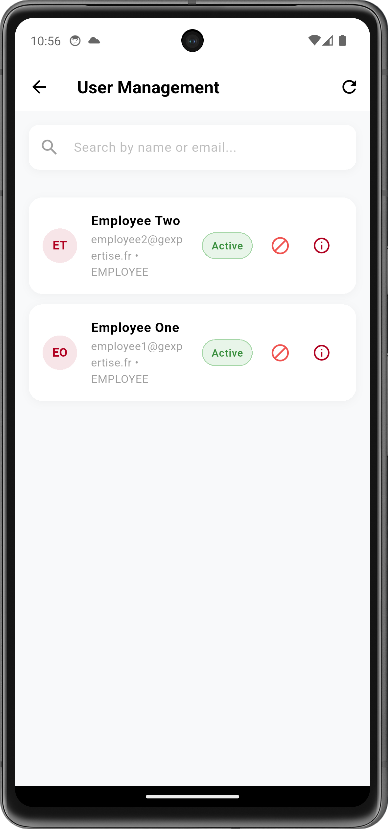
\includegraphics[width=0.3\textwidth]{images/ui/UserManagementInterface.png}
    \caption{User Management Interface}
\end{figure}

\section{Sprint Validation}

At the end of Sprint 1, a structured validation process was conducted to ensure that all implemented functionalities meet both functional and security requirements. This validation follows an Agile approach, where testing is performed incrementally at the end of each sprint to guarantee system reliability before progressing to subsequent development phases.

\subsection{Validation Objectives}

The validation process aims to:

\begin{itemize}
    \item Ensure correct behavior of authentication and access control mechanisms
    \item Verify enforcement of enterprise domain restrictions
    \item Validate user profile management operations
    \item Confirm proper functioning of administrative control features
\end{itemize}

\subsection{Test Scenarios}

The system was evaluated through a set of representative functional scenarios:

\begin{itemize}
    \item \textbf{Scenario 1: Successful Authentication} \\
    A user attempts to log in using a valid Office 365 account with an authorized domain. The system should authenticate the user and grant access to the platform.

    \item \textbf{Scenario 2: Unauthorized Domain Access} \\
    A user attempts to authenticate with an email address outside the \textbf{@gexpertise.fr} domain. The system must reject the request and display an appropriate error message.

    \item \textbf{Scenario 3: Profile Update Validation} \\
    An authenticated user updates profile information. The system must validate the input and persist the updated data correctly in the database.

    \item \textbf{Scenario 4: Administrative Control} \\
    An administrator performs actions such as monitoring user activity or restricting an account. The system must apply these changes consistently and reflect them immediately.
\end{itemize}

\subsection{Expected Results}

Each scenario is associated with expected outcomes:

\begin{itemize}
    \item Authorized users are successfully authenticated and redirected to the application
    \item Unauthorized users are denied access based on domain validation rules
    \item Profile updates are correctly validated and stored
    \item Administrative actions are enforced and reflected in system behavior
\end{itemize}

\subsection{Validation Outcome}

All defined scenarios were executed successfully, confirming that the system behaves as expected under both normal and exceptional conditions.

The validation results demonstrate that the authentication mechanism, user management features, and administrative controls are correctly implemented and aligned with system requirements.

Furthermore, the tested scenarios directly correspond to the interactions illustrated in the sequence diagram, ensuring consistency between system design and implementation.
\section{Conclusion}

This chapter detailed the implementation of user management and authentication functionalities, which form the core security layer of the platform. By combining enterprise authentication, role-based access control, and administrative supervision, the system ensures controlled and secure user interactions.

The next chapter focuses on the implementation of ride management and real-time communication functionalities.